\documentclass[10pt,landscape]{article}
\usepackage{multicol}
\usepackage{calc}
\usepackage{ifthen}
\usepackage[landscape]{geometry}
\usepackage{amsmath,amsthm,amsfonts,amssymb}
\usepackage{color,graphicx,overpic}
\usepackage{hyperref}
\usepackage[]{algorithm}
\usepackage[noend]{algpseudocode}


\pdfinfo{
  /Title (example.pdf)
  /Creator (TeX)
  /Producer (pdfTeX 1.40.0)
  /Author (Seamus)
  /Subject (Example)
  /Keywords (pdflatex, latex,pdftex,tex)}

% This sets page margins to .5 inch if using letter paper, and to 1cm
% if using A4 paper. (This probably isn't strictly necessary.)
% If using another size paper, use default 1cm margins.
\ifthenelse{\lengthtest { \paperwidth = 11in}}
    { \geometry{top=.5in,left=.5in,right=.5in,bottom=.5in} }
    {\ifthenelse{ \lengthtest{ \paperwidth = 297mm}}
        {\geometry{top=1cm,left=1cm,right=1cm,bottom=1cm} }
        {\geometry{top=1cm,left=1cm,right=1cm,bottom=1cm} }
    }

% Turn off header and footer
\pagestyle{empty}

% Redefine section commands to use less space
\makeatletter
\renewcommand{\section}{\@startsection{section}{1}{0mm}%
                                {-1ex plus -.5ex minus -.2ex}%
                                {0.5ex plus .2ex}%x
                                {\normalfont\large\bfseries}}
\renewcommand{\subsection}{\@startsection{subsection}{2}{0mm}%
                                {-1explus -.5ex minus -.2ex}%
                                {0.5ex plus .2ex}%
                                {\normalfont\normalsize\bfseries}}
\renewcommand{\subsubsection}{\@startsection{subsubsection}{3}{0mm}%
                                {-1ex plus -.5ex minus -.2ex}%
                                {1ex plus .2ex}%
                                {\normalfont\small\bfseries}}
\makeatother

% Define BibTeX command
\def\BibTeX{{\rm B\kern-.05em{\sc i\kern-.025em b}\kern-.08em
    T\kern-.1667em\lower.7ex\hbox{E}\kern-.125emX}}

% Don't print section numbers
\setcounter{secnumdepth}{0}


\setlength{\parindent}{0pt}
\setlength{\parskip}{0pt plus 0.5ex}

%My Environments
\newtheorem{example}[section]{Example}
% -----------------------------------------------------------------------

\begin{document}
\raggedright
\footnotesize
\begin{multicols}{3}


% multicol parameters
% These lengths are set only within the two main columns
%\setlength{\columnseprule}{0.25pt}
\setlength{\premulticols}{1pt}
\setlength{\postmulticols}{1pt}
\setlength{\multicolsep}{1pt}
\setlength{\columnsep}{2pt}

\begin{center}
     \Large{\underline{Cheat Sheet \#1}} \\
\end{center}

\section{Hello World}
\begin{algorithm}[H]
\caption{Hello World}
  \begin{algorithmic}
  \State \textbf{public static void} main()\\
  \{
  \State \hspace{10mm}System.out.println("Hello World!");\\
  \}
  \end{algorithmic}
\end{algorithm}

\section{Development}
\subsection{Editing}
Using IDE for features like
\begin{itemize}
\item Code Completion
\item Syntax checking
\item Refactoring
\item Automatic Code Generation
\end{itemize}
Common IDEs
\begin{itemize}
\item Eclipse
\item Netbeans
\item Intellij IDEA
\end{itemize}
\subsection{Compiling}
Using the compiler creates Bytecode out of sourcecode (.java $\rightarrow$  .out).\\
Use command line compiler \emph{javac} or IDE.\\
\subsection{Running}
Bytecode can be run in the Java VM.\\
Use command line \emph{java} or IDE.
\subsection{Debugging}
Jump into code at a certain point during runtime.\\
Set Breakpoints to specify debug entry points.\\
Observe current variable state.\\
Step through code line by line.\\
\section{Reserved Names}
There are round about 54 reserved names that cannot be used as identifiers in JAVA.
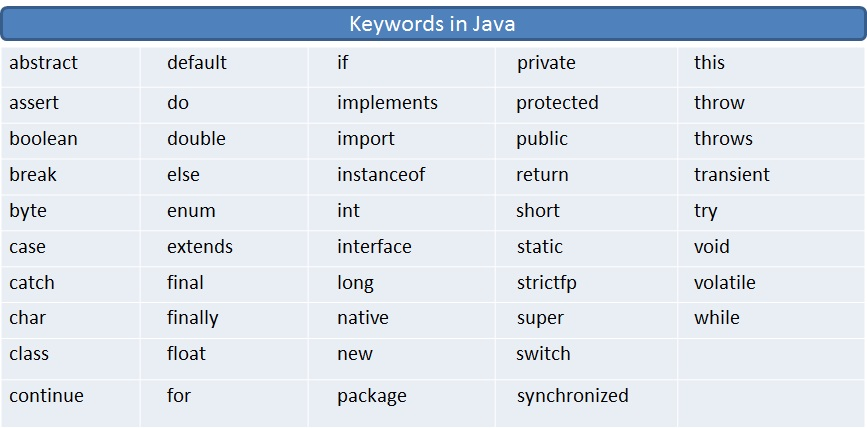
\includegraphics[scale=0.35]{keywords.png}\\
(http://www.f5java.com/images/java-tutorial-keywords-in-java.jpg)

\section{Naming Conventions}
\textbf{Package} names lower case.\\
\textbf{Class} names start capital, use CamelCase and describe the purpose of the class.\\
\textbf{Function} names start lower case, use CamelCase and describe its behavior.\\
\textbf{Variable} names start lower case and describe the data stored in the variable.\\
\textbf{Interface} names start capital, use CamelCase and describe an adjective the Interface provides.\\
\textbf{Constant} names have only capital letters and multiple words are separated by underscores.\\
Boolean \textbf{getters} have prefix "is", all other "get".\\
\textbf{Setters} have prefix "set".

\section{Program Layout}
\textbf{Packages} contain \emph{classes} or other \emph{packages}.\\
\textbf{Classes} contain \emph{variables} and \emph{functions}.\\
Every \emph{class} contains a \textbf{constructor}.\\
Only \emph{classes} containing a \textbf{main} method can be run.
\section{Comments}
\textbf{Inline Comments} $\rightarrow$ \emph{//}\\
\textbf{Multi Line Comments} $\rightarrow$ \emph{/* * */}\\
\textbf{JavaDOC} $\rightarrow$ \emph{/**  * */}\\
Try to avoid comments. If a code block has to be commented, \textbf{extract a method} with descriptive name instead.
Use JavaDOC on API (public methods).

\section{Coding conventions} 
There are no universal coding conventions. There are popular ones and rather specific ones. The important thing is to \textbf{agree on a set of rules} with your team!
\begin{itemize}
\item \textbf{Indentations} - use 2 spaces
\item Open \textbf{parenthesis} in new line
\item Use \textbf{Private Members} - use only getters and setters
\item Do not use \textbf{Parameters as return values}
\item Use \textbf{TDD} or at least \textbf{write tests} for each class afterwards
\item Use \textbf{empty lines} for vertical grouping of variables
\item Keep {classes} short $\rightarrow$ single responsibility
\item Keep {functions} short $\rightarrow$ A function should do one thing only 
\end{itemize}

% You can even have references
\rule{0.3\linewidth}{0.25pt}
\scriptsize
\bibliographystyle{abstract}
\bibliography{refFile}
\end{multicols}
\end{document}